


\begin{figure}[ht]
\centering
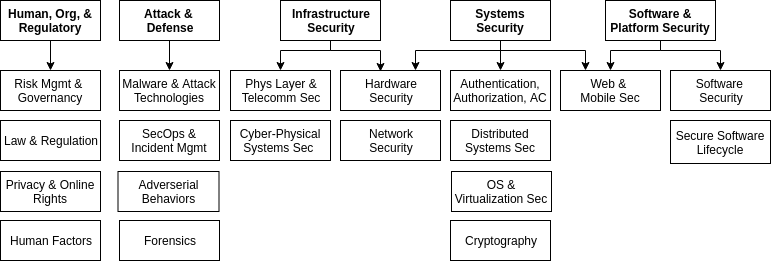
\includegraphics[width=.75\linewidth]{resource/img/ch_intro/taxonomies/cybok_vert_no_heading.png}
\caption{Cyber Security Body of Knowledge - Key Areas \cite{Rashid_Chivers_Danezis_Lupu_Martin}}
\label{fig:intro:cybok}
\end{figure} 


% \begin{figure}[ht]
% \centering
% 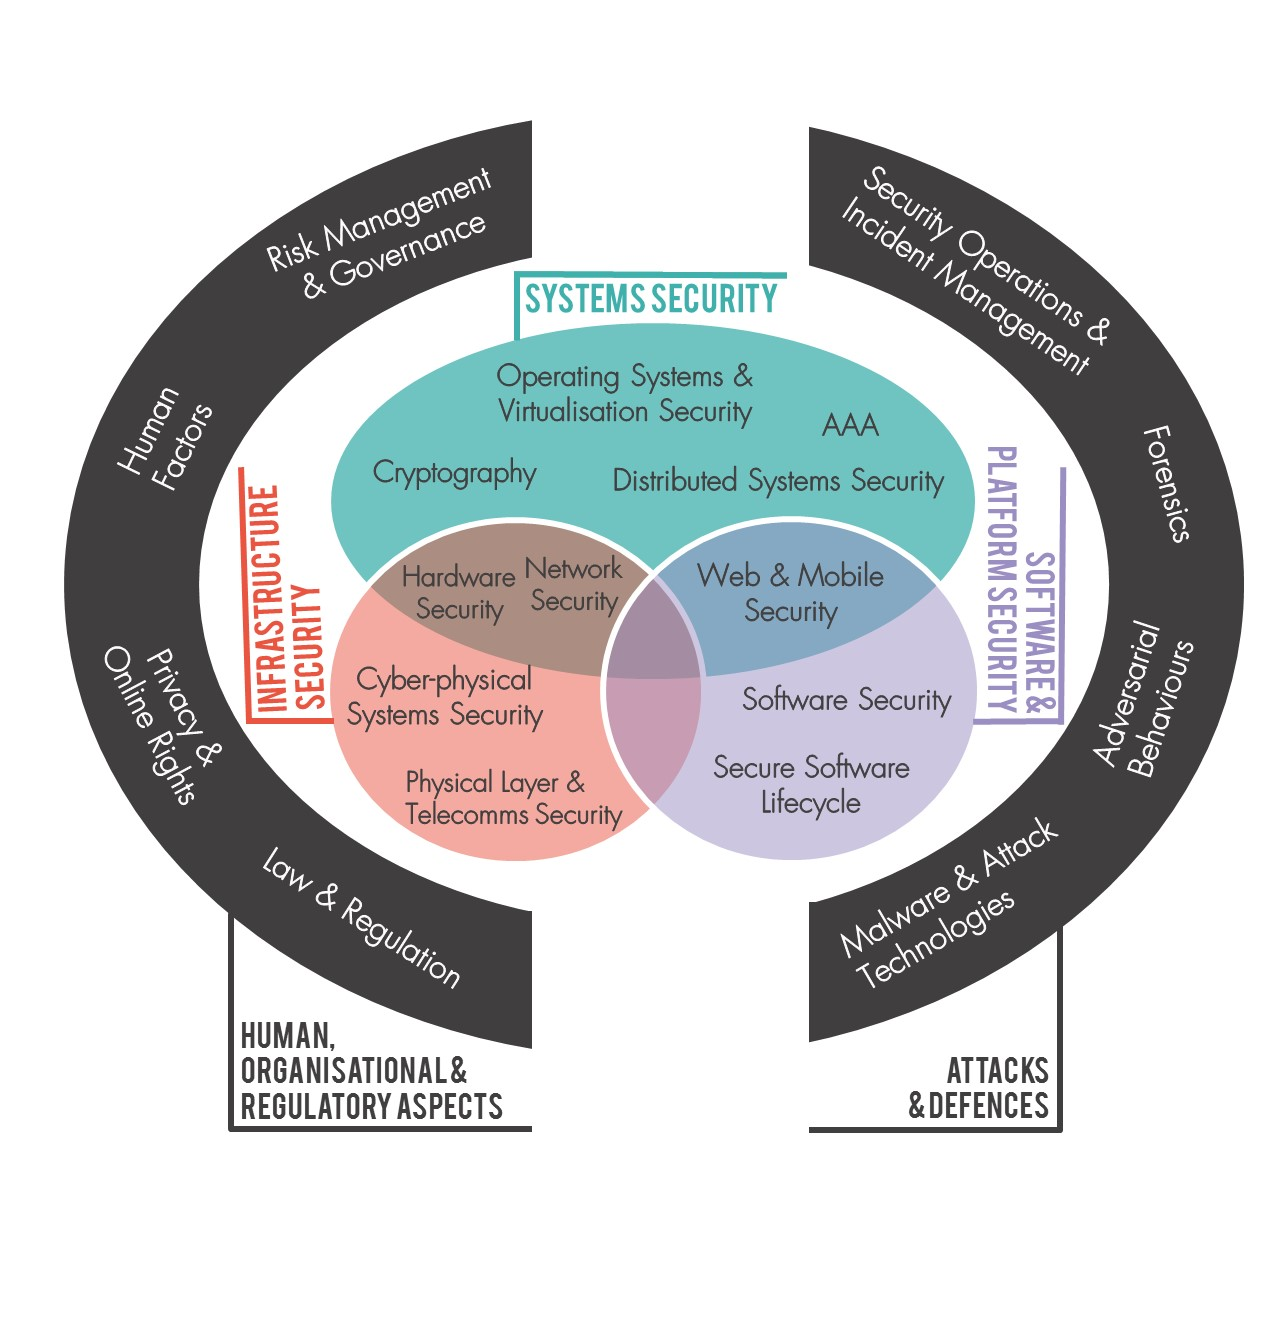
\includegraphics[width=.75\linewidth]{resource/img/ch_intro/CyBOK_clusters_-_Final.jpg}
% \caption{Cyber Security Body of Knowledge - Key Areas \cite{Rashid_Chivers_Danezis_Lupu_Martin}}
% \label{fig:intro:cybok}
% \end{figure} 

% Before discussing security metrics, we first take a step back to define what it is we intend to measure. 
Cyber security as a subject is at once broad and deep, covering a wide range of functional topics and skill sets. The lens through which a database administrator views security differs from that of a network engineer or an application developer within a particular business, and these perspectives may diverge from corresponding roles in other industry sectors. Thus, to effectively communicate any security objectives, it is necessary to understand the frame of reference from which they arise. In this work we refer to the Cyber Security Body of Knowledge\cite{Rashid_Chivers_Danezis_Lupu_Martin} (CyBoK) Key  Areas(KAs) as waypoints while navigating various aspects of security. The CyBoK project, sponsored by the UK's National Cyber Security Centre, provides both a taxonomy of cyber security topics, and a mapping to canonical references for these topics. Figure \ref{fig:intro:cybok} summarizes the 19 top level KAs and 5 broad categorical groupings.  Rather than delve into all the different CyBoK headings here in isolation, we elect instead to refer to the relevant classes as we encounter them in developing the thesis. 
%Finally, we provide working definitions for common terms found throughout this paper:

% Before discussing security metrics, we first take a step back to define what it is we intend to measure. 
% \begin{definition}
% \textbf{Metric}: The definition of a specific standard unit of measurement.
% \end{definition}
% \begin{definition}
% \textbf{Measurement}: A sampled value of a metric.
% \end{definition}
% \begin{definition}
% \textbf{Test}: The instrument and procedure used to obtain a measurement.
% \end{definition}
% \begin{definition}
% \textbf{Benchmark}: A standard environment and observed measurements for a metric.
% \end{definition}

Cyber security can be considered in terms of adversaries, along with their goals, and defenders, whose implicit goal is to prevent an adversary from achieving theirs. The purpose of a security metric is to quantify a specific aspect of cyber security, such as attacker
capabilities or defensive controls. We now frame the problem this work addresses by summarizing the security metrics and measurement techniques currently available, armed with the vocabulary and taxonomy needed to analyze them in context. 

\textbf{Regulatory and Compliance Metrics}: The left containing bracket in Figure \ref{fig:intro:cybok} depicts Human, Organizational, and Regulatory Aspects, and within the Risk Management KA\cite{Burnap_2019} we find the topic of security metrics. Indeed, security metrics are often defined within the scope of regulatory compliance. NIST's \textit{Security Metrics Guide for Information Technology Systems} \cite{Swanson_Bartol_Sabato_Hash_Graffo_2003,Chew_Swanson_Stine_Bartol_Brown_Robinson_2008}, ISO 27004 \textit{Monitoring, measurement, analysis and evaluation}\cite{iso_27004} and the Center for Internet Security's \textit{CIS Controls Measures \& Metrics}\cite{cis_cic} define the requirements for security metrics programs within various industry and government organisations. These security metrics are generally compliance focused, capturing statistics or percentages like employee training completion rate, number of hosts scanned and vulnerabilities found, or system performance complaints since the last patch roll out. 

\textbf{Operational Metrics} The right containing bracket in Figure \ref{fig:intro:cybok} labelled Attacks \& Defences includes security metrics listed in the \textit{Security Operations and Incident Response}\cite{Debar_2019} KA. The measurement processes in the operational area are distinguished primarily through automation support. Security Information and Event Management (SIEM) systems play a large role in collecting and aligning system telemetry for incident monitoring and response. SIEMs provide correlation of host/network event logs, IDS/IPS alerts, threat/vulnerability feeds, etc, and present a unified view of the system’s security posture automatically to the SOC. Before the advent of managed SIEMs, system administrators typically filled the role of security engineers, and relied on hand rolled collections of shell/perl scripts to manage systems, parse logs, collect or push events, format reports, and issue alarms.  To be effective required tribal knowledge along with proficiency in programming, network plumbing, and systems management, so changes to the environment or workforce made it extremely difficult(expensive) to deliver continuous monitoring capabilities to operators at any scale.  


\textbf{Vulnerability Metrics} Common to the 3 interior categories of Infrastructure, Systems, and Software \& Platform Security in Figure \ref{fig:intro:cybok} are vulnerability metrics. The Common Vulnerability Scoring System\cite{Mell07thecommon} (CVSS) is an open framework used throughout government and industry to report the severity of specific security vulnerabilities in commonly used software products. CVSS scores range from 0 to 10 based on the vulnerability’s exploitability and impact, with a score of 10 signifying the highest severity.  Exploitability is calculated by determining the access vector, access complexity, and number of authentication attempts required to exploit the vulnerability, with higher exploitability values equating to an easier compromise. Impact scores are determined by identifying the scope of a successful exploit on the vulnerable system’s confidentiality, integrity, and availability. 
%CVSS scores used in this research were queried using a local copy of the National Vulnerability Database (NVD) synchronized via MulVal's built-in mechanism and augmented with scores provided by vendors when an official Common Vulnerability Enumeration (CVE) designation was not available.  `


\begin{figure}[ht]
\centering
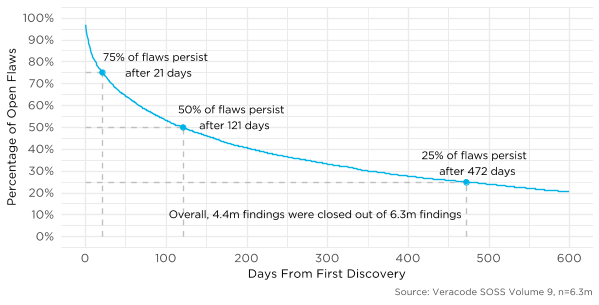
\includegraphics[width=.9\linewidth]{resource/img/ch_intro/veracode_closures_survival_analysis.png}
\caption{Veracode Static Analysis Remediation Times SOSS \cite{soss_v9}}
\label{fig:intro:soss-survival}
\end{figure} 


Static analysis\cite{Basili_Briand_Melo_1996} is a common method to identify possible vulnerabilities in software not included in the CVSS set. Developers can automatically scan custom source code and 3rd party libraries from within their IDE, or include hooks in their repository/CI to check incoming commits before merging. The metrics produced from static analysis can alert developers\cite{Johnson_2013} to common vulnerabilities in the code they write.  Figure \ref{fig:intro:soss-survival} shows the survival rate for static scan findings in 2018. 



\textbf{Economic Metrics} Measuring the trade-offs between competing interests and the incentives influencing actors is pervasive throughout cyber security. Security economics\cite{Anderson_2001} applies prevailing microeconomics models to describe limiting factors for attack and defense agents. The Gordon-Loeb\cite{Gordon_Loeb} model details an optimal security investment under the assumption of diminishing marginal returns.  In \textit{Security Metrics and Security Investment}\cite{Bohme_Moore} the authors derive metrics including the return on security investment (ROSI) and net present value (NPV) over future periods while accounting for different risk management temperaments. A survey of the economics of information security\cite{Anderson_Moore} literature summarizes potential applications of these economic metrics in many of the key cyber security areas. 


\begin{figure}[ht]
\centering
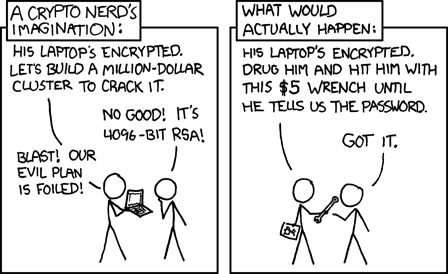
\includegraphics[width=.6\linewidth]{resource/img/ch_intro/xkcd_538_threat_model_econsec.png}
\caption{ source: https://www.xkcd.com/538/ }
\label{fig:intro:xkcd}
\end{figure} 

Figure \ref{fig:intro:xkcd} shows anecdotally one type of situation that economic metrics help us to avoid. Given an existing defensive capability that already deters attacks (data at rest cryptography in this case), further investment in that defense will give limited additional value. It also demonstrates the dangers of evaluating risk based on too narrow a security domain. Defining an attacker's capabilities, or threat modeling, is described in Section  \ref{sec:intro:threat_modeling}.


The evolution of information systems is trending away from a single administrative domain with a clear security boundary and moving towards a mix of self-hosted, provider managed, and remote 3rd party services. This creates unique challenges from an information security perspective, not least of which being how to define the new perimeter. 

% In order to evaluate the system's security posture in a mixed environment 

% while considering any architectural design changes made. Not only does this include a review of existing security controls, but also an assessment of the effects any regulatory compliance requirements will have on the deployment. Additionally, whereas a solution that resides totally in house can be evaluated in the context of a single security boundary, extending the perimeter to the public cloud requires an implicit acceptance that the cloud provider's administrative users have a higher privilege level than any tenant role that can be assigned. 

% A typical example being a company that maintains commercially sensitive data in house, but deploys access services to the public cloud and delegates authentication or authorization mechanics to vendors like Facebook or PayPal. 

